\documentclass[]{article}
\newcommand{\FileDepth}{../../..}
\usepackage[letterpaper, landscape, margin=0.5cm]{geometry}
\usepackage[T1]{fontenc}
\usepackage{textcomp}%Not strictly necessary, but gives \textmu command for "micro."
\usepackage{fancyhdr}
\usepackage{amsmath}
\usepackage{amssymb}
\usepackage{graphicx}
\usepackage{xcolor}
\usepackage{tikz}
\usetikzlibrary{calc}
\usepackage[shortlabels]{enumitem}
\usepackage{multicol}
\usepackage{vwcol}
\usepackage{hyperref}
\usepackage{wrapfig}
%opening
\newcommand{\SecType}{L}
\newcommand{\Week}{7}
\title{PH 211 Lecture \Week}
\author{Benjamin Bauml}
\date{Summer 2024}

\newcommand{\Purpose}{4}
\newcommand{\DefOnly}{0}

\input{\FileDepth/Formats/Assignment20240614.tex}
\usepackage[absolute]{textpos}
% This package relies on Assignment Format 2024-06-14 or later to work. It is recommended that the Purpose and DefOnly commands be given as such:
%\newcommand{\Purpose}{4}
%\newcommand{\DefOnly}{0}
% Activities need to be entered outside of the TeacherMargin and PresentSpace environments, otherwise they will be defined only locally. They can even go in the preamble.
\newenvironment{TeacherMargin}{\begin{textblock*}{10.8cm}(0.5cm,0.5cm)
\small}{\end{textblock*}
\hspace{0.1cm}}
\newenvironment{PresentSpace}{\begin{textblock*}{0.3cm}(26.85cm,9.35cm)
--
\end{textblock*}
\begin{textblock*}{15.6cm}(11.8cm,0.5cm)
\begin{Repurpose}{1}
\Large}{\end{Repurpose}
\end{textblock*}
\hspace{0.1cm}}

%\newcommand{\FBDaxes}[4][2]{
	\begin{scope}[shift={(#2)},rotate=#3]
		% x-axis
		\draw[thick,->] (-#1,0) -- (#1,0);
		\node[anchor=west] at (#1,0) {$x$};
		% y-axis
		\draw[thick,->] (0,-#1) -- (0,#1);
		\node[anchor=south] at (0,#1) {$y$};
		\coordinate (#4) at (0,0);
	\end{scope}
}
\newcommand{\FBDvectorMA}[4]{
	\begin{scope}[shift={(#1)}]
		\coordinate (#4tip) at ({#2*cos(#3)},{#2*sin(#3)});
		\draw[ultra thick,blue,->] (#1) -- (#4tip);
	\end{scope}
}
\newcommand{\FBDvectorXY}[3]{
	\begin{scope}[shift={(#1)}]
		\coordinate (#3tip) at (#2);
		\draw[ultra thick,blue,->] (0,0) -- (#3tip);
	\end{scope}
}
\newcommand{\FBDdot}[1]{
	\filldraw[black] (#1) circle (3pt);
}
\newcommand{\FBDbox}[5][1]{
	\begin{scope}[shift={(#2)},rotate=#3]
		\filldraw[color=black,fill=white,thick] ({-#1/2},{#1/2}) -- ({-#1/2},{-#1/2}) -- ({#1/2},{-#1/2}) -- ({#1/2},{#1/2}) -- cycle;
		% Left side coordinates
		\coordinate (#4ltq) at ({-#1/2},{#1/4});
		\coordinate (#4lcent) at ({-#1/2},0);
		\coordinate (#4lbq) at ({-#1/2},{-#1/4});
		% right side coordinates
		\coordinate (#4rtq) at ({#1/2},{#1/4});
		\coordinate (#4rcent) at ({#1/2},0);
		\coordinate (#4rbq) at ({#1/2},{-#1/4});
		% top coordinates
		\coordinate (#4tlq) at ({-#1/4},{#1/2});
		\coordinate (#4tcent) at (0,{#1/2});
		\coordinate (#4trq) at ({#1/4},{#1/2});
		% bottom coordinates
		\coordinate (#4blq) at ({-#1/4},{-#1/2});
		\coordinate (#4bcent) at (0,{-#1/2});
		\coordinate (#4brq) at ({#1/4},{-#1/2});
		% corners
		\coordinate (#4tl) at ({-#1/2},{#1/2});
		\coordinate (#4tr) at ({#1/2},{#1/2});
		\coordinate (#4bl) at ({-#1/2},{-#1/2});
		\coordinate (#4br) at ({#1/2},{-#1/2});
		\node at (0,0) {#5};
	\end{scope}
}
%\newcommand{\MVec}[3][0]{%Creates a momentum vector of length #3 centered at #2 and rotated #1 degrees counterclockwise.
	\begin{scope}[rotate=#1,shift={(#2)}]
		\draw[->,thick] ({-#3/2},0) -- ({#3/2},0);
	\end{scope}
}
\newcommand{\MDot}[1]{%Creates a dot at #1 to represent a zero vector.
	\filldraw (#1) circle (1pt);
}
\newcommand{\MVDRows}[2][4.5]{%Creates the rows (initial, delta, final) of a momentum vector diagram. The optional argument determines the width of the table, and defaults to a good length for three columns (two objects and the total system). The non-optional argument gives a coordinate name (not displayed) to the diagram.
	\begin{scope}
		%\draw[thick] (0,5.5) -- (0,0);
		\draw[thick] (-1,4.5) -- (#1,4.5);
		\node at (-0.5,3.75) {$\vec{p}_{i}$};
		\draw[thick] (-1,3) -- (#1,3);
		\node at (-0.5,2.25) {$\Delta\vec{p}$};
		\draw[thick] (-1,1.5) -- (#1,1.5);
		\node at (-0.5,0.75) {$\vec{p}_{f}$};
		\coordinate (#2) at (0,5);
	\end{scope}
}
\newcommand{\MVDCol}[4][0.75]{%Creates a column for an object in a momentum vector diagram. The first (non-optional) argument is the coordinate name (not displayed) of the column, while the second is the displayed column header. The first argument also names the three entries down the column. The third argument anchors the column, so it should either be the coordinate name of the MVD (for the first column) or the coordinate name of the previous column. The optional argument indicates how far the center of the column should be from the previous column's edge, and defaults to 0.75.
	\begin{scope}[shift={(#4)}]
		\node at (#1,0) {#3};
		%\draw[thick] ({#1*2},0.5) -- ({#1*2},-5);
		\draw[thick] (0,0.5) -- (0,-5);
		\coordinate (#2init) at (#1,-1.25);
		\coordinate (#2delt) at (#1,-2.75);
		\coordinate (#2fin) at (#1,-4.25);
		\coordinate (#2) at ({#1*2},0);
	\end{scope}
}

%\input{\FileDepth/Activities/Activity_One/Activity_One.tex}
%\input{\FileDepth/Activities/Activity_Two/Activity_Two.tex}

\begin{document}
\begin{TeacherMargin}

\end{TeacherMargin}
\begin{PresentSpace}
\begin{center}
	\huge Lecture 7: Projectile Motion II
\end{center}
\vspace{0.5cm}
\underline{Warm-Up Activity} \\
Which of these equations are valid for an object moving with constant acceleration? Choose all that apply, and WRITE BIG!
%\begin{multicols}{2}
\begin{enumerate}[(A)]
	\item $\vec{a}(t)=a\hat{x}$
	%\vspace{6pt}
	\item $\vec{v}(t) = \left[v_{i}+a_{0}\left(t-\frac{t^{2}}{T}\right)\right]\hat{x}$
	%\vspace{15pt}
	\item $v_{f}^{2}=v_{i}^{2}+2a\Delta x$
	\item $\vec{x}(t) = \left[x_{i}+v_{i}t+\frac{1}{2}at^{2}\right]\hat{x}$
	\item None of the above.
\end{enumerate}
%\end{multicols}
\end{PresentSpace}
\newpage
\begin{TeacherMargin}

\end{TeacherMargin}
\begin{PresentSpace}
\textbf{A Model for Motion}
\begin{multicols}{2}
	Quantities
	\begin{itemize}
		\item Position: $\vec{r}$
		\item Velocity: $\vec{v}=\frac{d\vec{r}}{dt}$
		\item Acceleration: $\vec{a}=\frac{d\vec{v}}{dt}$
	\end{itemize}
	\vspace{1cm}
	Assumptions
	\begin{itemize}
		\item Use the Particle Model
	\end{itemize}
\end{multicols}
Motion Diagram
\begin{figure}[h]
	\centering
	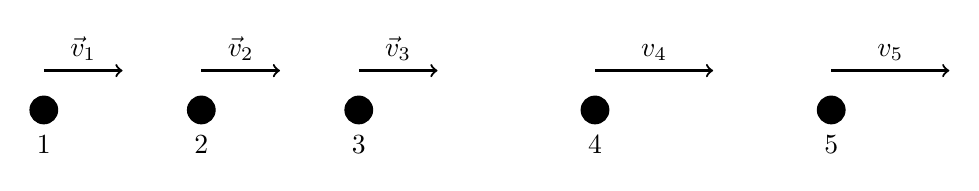
\begin{tikzpicture}
		\foreach \x in {1,2,3}
		\filldraw (2*\x,0) circle (5pt);
		\foreach \x in {1,2,3}
		\node[anchor=north] at (2*\x,-0.2) {\x};
		\foreach \x in {1,2,3}
		\draw[thick,->] (2*\x,0.5) -- (2*\x+1,0.5);
		\foreach \x in {1,2,3}
		\node[anchor=south] at (2*\x+0.5,0.5) {$\vec{v}_{\x}$};
		\begin{scope}[shift={(-3,0)}]
			\foreach \x in {4,5}
			\filldraw (3*\x,0) circle (5pt);
			\foreach \x in {4,5}
			\node[anchor=north] at (3*\x,-0.2) {\x};
			\foreach \x in {4,5}
			\draw[thick,->] (3*\x,0.5) -- (3*\x+1.5,0.5);
			\foreach \x in {4,5}
			\node[anchor=south] at (3*\x+0.75,0.5) {$v_{\x}$};
		\end{scope}
	\end{tikzpicture}
\end{figure}
\end{PresentSpace}
\newpage
\begin{TeacherMargin}
\noindent To smoothly derive the third kinematics equation, start with
\[
v_{f} = v_{i} + at,
\]
and square it to get
\[
v_{f}^{2} = v_{i}^{2} + 2v_{i}at + a^{2}t^{2}.
\]
You can factor out $2a$ from the last two terms to get
\[
v_{f}^{2} = v_{i}^{2} + 2a\left(v_{i}t + \frac{1}{2}at^{2}\right).
\]
Now you can substitute
\[
\Delta y = v_{i}t + \frac{1}{2}at^{2}
\]
cleanly into the prior equation to give
\[
v_{f}^{2} = v_{i}^{2} + 2a\Delta y.
\]
\end{TeacherMargin}
\begin{PresentSpace}
\vspace{-10pt}
\section*{Constant Acceleration}
\vspace{-10pt}
The \textit{constant-acceleration} equations (kinematics):
\begin{itemize}
	\item $a(t)=a$
	\item $v(t)=v_{i}+at$
	\item $x(t) = x_{i}+v_{i}t+\frac{1}{2}at^{2}$
\end{itemize}
\end{PresentSpace}
\newpage
\begin{TeacherMargin}
\noindent\textbf{Assumptions}
\begin{itemize}
	\item Particle Model
	\item 1-D Motion
	\begin{itemize}
		\item We will not complicate our calculations by worrying about minor amounts of horizontal motion, instead assuming all motion is vertical.
	\end{itemize}
	\item Near Earth
	\begin{itemize}
		\item Near the surface of Earth, acceleration due to gravity is approximately constant, so we can use the constant acceleration equations to describe the motion.
	\end{itemize}
\end{itemize}
\textbf{Interesting Quantities}
\begin{itemize}
	\item How long does it take to hit the water?
	\item How fast is the rock moving when it hits the water?
\end{itemize}
\begin{center}
	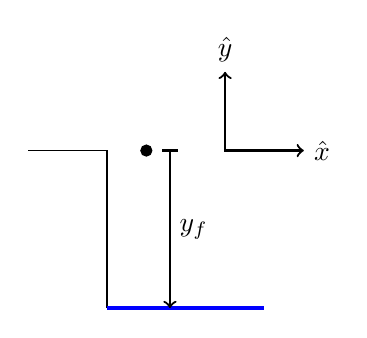
\begin{tikzpicture}
		\draw (0,0) -- (1,0) -- (1,-2);
		\draw[ultra thick, blue] (1,-2) -- (3,-2);
		\filldraw (1.5,0) circle (2pt);
		\begin{scope}[shift={(1.8,0)}]
			\draw[thick] (-0.1,0) -- (0.1,0);
			\draw[thick,->] (0,0) -- (0,-2);
			\node[anchor=west] at (0,-1) {$y_{f}$};
		\end{scope}
		\begin{scope}[shift={(2.5,0)}]
			\draw[thick,<->] (0,1) node[anchor=south] {$\hat{y}$} -- (0,0) -- (1,0) node[anchor=west] {$\hat{x}$};
		\end{scope}
	\end{tikzpicture}
\end{center}
\textbf{Identify Quantities by Symbol and Number}
\begin{align*}
	y_{i} & = 0\text{ m} & v_{i} & = 0\text{ m} & \vec{a}(t) & = -g\hat{y} \\
	y_{f} & = -45\text{ m} & v_{f} & = ? & g & = 9.81\text{ m/s}^{2} \approx 10\text{ m/s}^{2}
\end{align*}
\textbf{Symbolic Solution} \\
First, note that the kinematics equation for $y(t)$ simplifies quite a lot, as $y_{i}$ and $v_{i}$ are both zero:
\[
y(t) =  -\frac{g}{2}t^{2}.
\]
At $t_{f}$, we can rearrange this to find that
\[
t_{f} = \sqrt{-\frac{2y_{f}}{g}}
\]
This time is the only thing we are missing from the velocity kinematics equation:
\[
v_{f} = v_{i} - gt_{f} = -g\sqrt{-\frac{2y_{f}}{g}} = -\sqrt{-2gy_{f}}.
\]
\textbf{Plug in Numbers}
\begin{align*}
	v_{f} & = -\sqrt{-2(10\text{ m/s}^{2})(-45\text{ m})} = -\sqrt{900\text{ m}^{2}/\text{s}^{2}} = -30 \text{ m/s} \\
	t_{f} & = \sqrt{\frac{-2(-45\text{ m})}{10\text{ m/s}^{2}}} = \sqrt{9\text{ s}^{2}} = 3\text{ s}
\end{align*}
\end{TeacherMargin}
\begin{PresentSpace}
\vspace{-10pt}
\section*{L5-1: A Falling Rock}
\vspace{-10pt}
You drop a rock from a bridge that is 45 m above the water.
\begin{itemize}
	\item What assumptions should we make about the motion?
	\item What interesting quantities can we ask about?
\end{itemize}
\end{PresentSpace}
\newpage
\begin{TeacherMargin}
\noindent What if the acceleration in one direction is equal to zero? For constant acceleration, we can always turn our coordinate axes such that one axis (usually the $y$-axis) points along the acceleration vector, reducing our equations to:
\begin{align*}
	a_{x}(t) & = 0 & a_{y}(t) & = a_{y} \\
	v_{x}(t) & = v_{ix} & v_{y}(t) & = v_{iy}+a_{y}t \\
	x(t) & = x_{i}+v_{ix}t & y(t) & = y_{i}+v_{iy}t+\frac{1}{2}a_{y}t^{2}
\end{align*}
What if the acceleration in the $y$-direction is only due to gravity?
\begin{align*}
	a_{x}(t) & = 0 & a_{y}(t) & = -g \\
	v_{x}(t) & = v_{ix} & v_{y}(t) & = v_{iy}-gt \\
	x(t) & = x_{i}+v_{ix}t & y(t) & = y_{i}+v_{iy}t-\frac{1}{2}gt^{2}
\end{align*}
This assumes that $\hat{y}$ points upward, away from the surface of the Earth. We could choose a coordinate system such that down is positive, which would make $a_{y}(t) = g$.

\noindent NOTE: $g\approx9.81$ m/s$^{2}$. The negative sign comes from the coordinate system, not the definition of the constant!
\end{TeacherMargin}
\begin{PresentSpace}
\vspace{-10pt}
\section*{Acceleration in Two Dimensions}
\vspace{-10pt}
\begin{itemize}
	\item What if we have an object that moves (with constant acceleration) in two directions?
	\item We can treat the motion in each direction independently!
\end{itemize}
\begin{align*}
	a_{x}(t) & = a_{x} & a_{y}(t) & = a_{y} \\
	v_{x}(t) & = v_{ix}+a_{x}t & v_{y}(t) & = v_{iy}+a_{y}t \\
	x(t) & = x_{i}+v_{ix}t+\frac{1}{2}a_{x}t^{2} & y(t) & = y_{i}+v_{iy}t+\frac{1}{2}a_{y}t^{2}
\end{align*}
\begin{itemize}
\item What if the acceleration in one direction is equal to zero?
\item What if the acceleration in the $y$-direction is only due to gravity?
\end{itemize}
\end{PresentSpace}
\newpage
\begin{TeacherMargin}
\noindent\textbf{(1)}
\begin{center}
	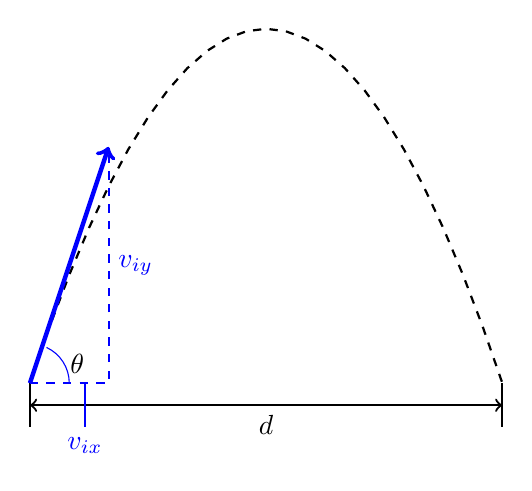
\begin{tikzpicture}[scale=2]
		\foreach \x in {0,3}
			\draw[thick] (\x,0) -- (\x,-8pt);
		\draw[thick,<->] (0,-4pt) -- (3,-4pt);
		\node[anchor=north] at (1.5,-4pt) {$d$};
		\draw[thick,dashed,domain=0:3,variable=\x] plot (\x,3*\x-\x*\x);
		\draw[ultra thick,blue,->] (0,0) -- (0.5,1.5);
		\draw[thick,dashed,blue] (0,0) -- (0.5,0) -- (0.5,1.5);
		\draw[blue] (0.25,0) arc (0:65:0.25);
		\node[anchor=south] at (0.30,0) {$\theta$};
		\draw[blue] (0.35,0) -- (0.35,-8pt) node[anchor=north] {$v_{ix}$};
		\node[blue,anchor=west] at (0.5,0.75) {$v_{iy}$};
	\end{tikzpicture}
\end{center}
\begin{multicols}{2}
From the picture, we can determine that $v_{ix} = v\cos\theta$ and $v_{iy} = v\sin\theta$.

\noindent\textbf{Identify Quantities by Symbol and Number}
\begin{align*}
	v_{i} & = v & t_{i} & = 0 & x_{i} & = 0 \\
	v_{f} & = ? & t_{f} & = ? & x_{f} & = d
\end{align*}

\noindent\textbf{(2)} \\
First, if we make the simplifying assumption that the rock starts and lands at the same height (ignoring the initial height from the person), then we can use $y_{i} = y_{f}$ write
\begin{align*}
	y_{f} & = y_{i}+v_{iy}t-\frac{1}{2}gt^{2} \\
	0 & = 0 + v\sin\theta t - \frac{1}{2}gt^{2} \\
	\frac{1}{2}gt^{2} & = v\sin\theta t
\end{align*}
Thus, the time of flight is
\[
t_{\text{ToF}} = \frac{2v\sin\theta}{g}.
\]
We also know that the rock travels a distance $d$ over the course of the time of flight, so
\begin{align*}
	x_{f} & = x_{i}+v_{ix}t \\
	d & = v\cos\theta t_{\text{ToF}}.
\end{align*}
This gives us a second equation for time of flight,
\[
t_{\text{ToF}} = \frac{d}{v\cos\theta},
\]
which together with our previous expression gives us
\[
\frac{2v\sin\theta}{g} = \frac{d}{v\cos\theta},
\]
which may be useful in relating many different quantities.

\noindent\textbf{(3)} \\
At the highest point, $v_{y} = 0$ (and $v_{x}=v$). At the time it takes to reach the peak, we have
\begin{align*}
	v_{y}(t_{\text{peak}}) & = v_{iy} - gt_{\text{peak}} \\
	0 & = v\sin\theta - gt_{\text{peak}} \\
	t_{\text{peak}} & = \frac{v}{g}\sin\theta.
\end{align*}
The peak occurs half way through the motion ($t_{\text{peak}}=\frac{1}{2}t_{\text{ToF}}$)!
\end{multicols}
\end{TeacherMargin}
\begin{PresentSpace}
	\vspace{-10pt}
	\section*{L5-2: A Thrown Rock}
	\vspace{-10pt}
	\begin{itemize}
		\item You throw a rock across a flat field.
		\item The rock's initial speed is $v$, thrown at an angle $\theta$ above the horizontal.
		\item The rock lands a distance $d$ away from you.
		\begin{enumerate}[(1)]
			\item Sketch a diagram to help you find the $x$- and $y$-components of the rock's velocity in terms of $v$ and $\theta$.
			\item Write an equation that would allow you to find the amount of time that the ball is in the air.
			\item How is this time related to the amount of time the ball takes to reach its highest point above the ground?
		\end{enumerate}
	\end{itemize}
\end{PresentSpace}
\newpage
\begin{TeacherMargin}

\end{TeacherMargin}
\begin{PresentSpace}
\section*{Main Ideas}
\begin{itemize}
	\item We can use the kinematics equations to solve for any quantity of interest when the acceleration is constant.
	\item Motion in 2 dimensions can be broken down into independent motion in each dimension.
\end{itemize}
\end{PresentSpace}
\end{document}